\documentclass{article}
\usepackage[francais]{babel}
\usepackage[utf8]{inputenc}  
\usepackage[T1]{fontenc} 
\usepackage{multirow}
\usepackage{footnote}
\usepackage{longtable}
\usepackage{graphicx}

\usepackage[top=2cm, bottom=2.5cm, left=1.5cm, right=1.5cm]{geometry}

\title{Système Digital\\Rapport de projet}
\author{Elie Michel, Louis Garrigue, Nicolas Jeannerod et Aurélien Delobelle}
\date{27 janvier 2013}

\begin{document}

\maketitle

\section{Vue d'ensemble}

\begin{figure}[h]
\centering
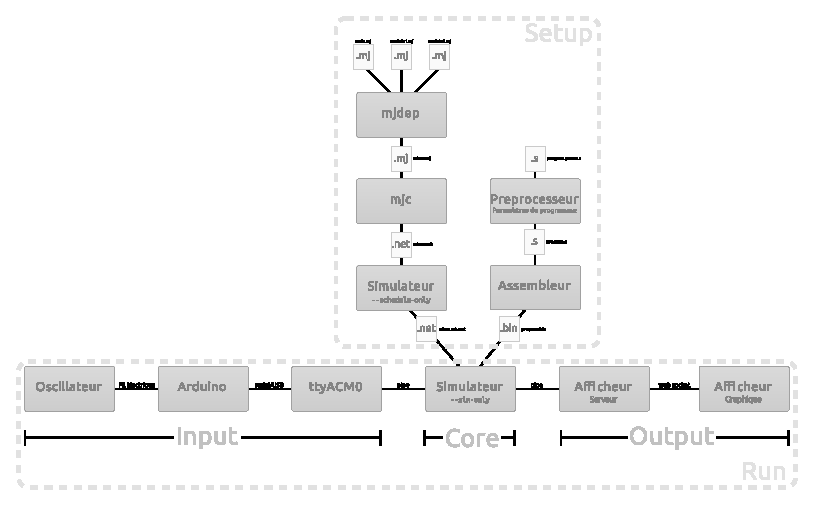
\includegraphics{organisation.eps}
\caption{\label{orga} Organisation du projet}
\end{figure}
\paragraph{}Le but principal de ce projet est la conception d'un microprocesseur, mais c'est autour du simulateur que le projet s'organise, comme le montre la figure \ref{orga}.

\paragraph{}Ce simulateur reçoit des informations de trois types différents :
\begin{itemize}
	\item Le circuit à simuler
	\item L'état de la ROM (le programme, dans le cas de notre microprocesseur)
	\item Les entrées du circuit
\end{itemize}

\paragraph{}Il retourne ensuite les sorites du circuit. Il est intéressant de faire la distinction entre les entrées/sorties du circuit, qui se font en temps réel lors de la simulation et le chargement du circuit et de la ROM qui se font à l'initialisation, depuis des fichiers préalablement générés. Ces deux phases sont appelées respectivement `run` et `setup` et possèdent chacune un script éponyme à la racine de l'archive.


\paragraph{}Le simulateur lui-même peut également se décomposer en plusieurs phases :
\begin{itemize}
	\item Le parseur de netlist
	\item L'optimizer, qui ordonne et simplifie les netlists
	\item Le parseur de fichier de ROM
	\item L'initialisation, convertissant l'AST en structure plus adaptée à la simulation
	\item Le cœur du simulateur
\end{itemize}


\paragraph{}Le microprocesseur est construit en utilisant minijazz et un préprocesseur permettant l'agrégation de plusieurs fichiers. Le programme est assemblé par le programme jupiter. L'entrée du circuit est reliée par l'intermédiaire du port série à un oscillateur carré réel et la sortie peut être reliée à deux afficheurs, l'un graphique et l'autre non.



\section{Simulateur}



\section{Microprocesseur}
\subsection{Introduction}

Nous avons commencé par nous baser sur le fonctionnement des microprocesseurs
MIPS étant donné que c'était la seule architecture que nous connaissions.
Nous avons cependant tenu à faire quelque chose de différent.

\subsubsection{Ligne de conduite}
Notre premier choix important a été de décider que chaque fonction du
microprocesseur prendrait ses arguments dans les mêmes registres prévus à cet effet
(à savoir les \$a*), et renverrait ses résultats dans les registres prévus à
cet effet (les \$r*), à l'instar des appels système de MIPS qui regardent
toujours \$v0 et \$a0.

\subsubsection{Densité}
Ce choix nous a dirigé vers un objectif de densité. Nous avons alors constaté
qu'il était possible de ne conserver que 4 registres
\footnote{\$a0, \$a1, \$r0, \$r1}, réduisant par là énormément le nombre
d'instructions de gestion de la mémoire puisque nous n'avions donc  plus besoin
que de 2 bits pour choisir un registre.

Nous avons au début cherché la densité maximale, avec un très petit jeu
d'instructions (sur 5 bits seulement !).
Mais pour des raisons pratiques (pour que certaines manipulations ne prennent pas
trop d'instructions) nous l'avons enrichi. Finalement, les instructions sont
codées sur 6 bits.


\subsection{Architecture générale}

\subsubsection{Taille des valeurs}
Le choix de la taille en bit des valeurs manipulées par le microprocesseur est
un choix important et l'un des premiers que l'on ait fait. Il nous fallait trouver
un compromis entre petite taille et maniabilité.

Les valeurs à afficher dans l'horloge sont toutes, à l'exception de l'année, de
taille inférieure à 256 et le choix de mots de 8 bits nous ont semblés être un
choix raisonnable. Pour la gestion des années, nous avons choisi de découper en
deux bytes selon son écriture décimale et non binaire afin de simplifier la
conversion en 7 segments.

Ce choix a par la même occasion déterminé le nombre de cases mémoire puisque nous utilisons un registre pour choisir l'adresse. Une RAM de 256 adresses est largement suffisante pour programmer une horloge. Nous sommes cependant revenu sur ce choix par la suite. (\emph{cf}~\ref{micro_update})

\paragraph{Dans la ROM}
Il n'était par contre pas possible de se limiter à des programmes de 256 instructions
seulement, d'autant plus que notre jeu d'instructions extrêmement bas niveau nous
oblige à produire de longs programmes. Le curseur d'instructions est donc représenté
sur 16 bits, permettant des programmes de 65 636 instructions. Cette disparité
entre la taille des mots machine et celle du curseur d'instructions nous a contraint
à utiliser des sauts de taille relative plutôt qu'absolue. Il est cependant toujours
possible de spécifier des tailles absolues dans des cas où c'est nécessaire en
utilisant deux registres.

\subsubsection{Séparation en unités}
Nous avons séparé les instructions en 4 unités en fonction de leurs
deux premiers bits en langage machine :
\begin{itemize}
  \item SYS qui s'occupe des entrées et sorties de la machine (depuis
    l'horloge, et vers l'affichage).
  \item ALU qui fait les opérations de base, arithmétiques et logiques (add,
    sub, mult, div\footnote{La division est euclidienne} ; and, or, not, shift).
  \item MEM qui gère les accès mémoire, que ce soit entre registres ou entre un
  registre et la RAM.
  \item JUMP qui contrôle l'adresse de lecture des instructions.
\end{itemize}

\paragraph{Inconvénients}
La séparation en quatre unité impose un nombre fixe d'instructions possibles
par unité, ce qui a amené quelques choix discutables :
\begin{itemize}
  \item Par manque de place, le move d'un \$a[i] vers un \$a[j]
    (resp. \$r[i] vers \$r[j]) n'existe pas. On doit pour cela utiliser une
    étape intermédiaire.
  \item Nous avions absolument besoin du LI (load immediate), et ne trouvions
    pas de place pour cette instruction. Finalement, elle appartient à l'ALU.
  \item Pour certaines instructions, on ne peut regarder que dans \$a0 (et \$a1
    si deux arguments sont exigés), alors que pour d'autres on peut choisir
    le(s) registre(s) d'argument(s). Cela est dû au fait que certaines unités
    manquaient de place par rapport à d'autres.
  \item L'unité JUMP a accueilli les commandes WCA (Write Current Adress) et
    END (termine le programme)
\end{itemize}


\subsubsection{Notes sur le load immediat}
Le LI est une instruction qui nous a posé problème car elle est contradictoire
avec la petite taille de nos instructions. En effet, l'instruction doit contenir
la valeur que l'on veut charger, ce qui n'est pas possible avec des instructions
plus petites que les mots machine.

\paragraph{}
Une première idée fut d'interpréter l'instruction suivante non pas comme une
instruction mais comme une valeur. En utilisant les 2 derniers bits de l'instruction
LI puis les 6 bits de l'instruction suivante, on pouvait charger toute valeur.

Le problème est que cela revenait en fait à faire des instructions de taille variable
et complexifiait le processeur. Gérer des tailles variables pour une seule instruction
manquait de cohérence et nous avons préféré faire un chargement partiel, ne gérant
pas toutes les valeurs possibles.

\paragraph{}
Il s'est ensuite posé la question du choix valeurs à gérer. La réponse la plus immédiate
est de charger les bits de poids faible seulement. Une autre solution aurait
pu être de choisir des valeurs que l'on est plus susceptible d'utiliser pour l'horloge,
comme 24 ou 60, mais nous préfèrions conserver un minimum de généralité. Il était
également possible de choisir les nombres premiers pour simplifier la décomposition
en sous-étapes du chargement de valeurs plus importantes, mais nous n'avions la place
dans le jeu d'instruction de ne choisir que 8 valeurs et en ajoutant 0 et 1 on ne
pouvait aller que jusqu'à 11 (ou 13 sans 0), ce qui ne permet pas de décomposer
tout nombre représenté sur 8 bits. Finalement, nous avons donc conservé la première
solution.

\subsubsection{Notes sur le shift}
Une autre instruction à laquelle notre choix de densité a donné un comportement
particulier est le shift. On ne choisi pas à l'appel de cette fonction le sens dans
lequel se fait le décalage et pour cause, il se fait toujours vers les poids forts.
Si on veut faire un décalage de $n$ vers les poids faibles, il suffit en fait de
faire un décalage de $8 - n$ puis de regarder les poids forts du résultat seulement
(c'est-à-dire le registre \$r1).

\subsubsection{Notes sur les sauts conditionnels}
La densité joue également un rôle dans le fonctionnement des sauts conditionnels.
Plutôt que de faire une instruction \emph{branch if equal zero} prenant en argument
à la fois une adresse et un registre à tester, on ne regarde qu'un registre et on
laisse le choix du type (avant/arrière, absolu/relatif) et de l'amplitude du saut
à l'instruction suivante.

Une amélioration que nous pourions envisager dans les instructions de saut est
l'ajout de sauts de taille fixe. Il y a à cela deux raisons :
\begin{itemize}
  \item Les instructions de saut relatif permettent de choisir un registre, contrairement
        à la philosophie que nous voulions adopter. C'est uniquement dû au fait qu'il
        restait de la place dans le jeu d'instructions de l'unité JUMP mais on pourait
        parfaitement envisager de retirer certaines de ces instructions.
  \item Les sauts relatifs sont le cas le plus courant où il est nécessaire de charger
        une constante écrite sur plus de 3 bits et est donc fastidieux à programmer.
        Il serait donc bien plus simple d'avoir une instruction faisant un « grand »
        saut, même s'il est de taille fixe car on peut alors au besoin ajouter des
        instructions vides pour ajuster le répéter.
\end{itemize}

Il est à noter que ce comportement peut être simulé en enregistrant dans une case
mémoire facilement accessible (entre 0 et 7, pour qu'un LI suffise à charger son
adresse) une valeur élevée dès le début du programme, on peut émuler cette fonctionnalité.

\subsubsection{Stockage de la date/heure}
Nous imaginions d'abord réserver des adresses particulières de la RAM pour
stocker les valeurs de la date/heure. Le problème de cette méthode est que l'on
ne peut faire qu'un seul accès simultané à la RAM et il n'était donc pas possible
d'afficher ces valeurs en même temps. Nous avons donc utilisé une mémoire
spécifique : 7 registres en écriture seule branchés à la sortie font office
de mémoire graphique.

\paragraph{}
Ces registres ne peuvent cependant pas être modifiés simultanément, du fait de
notre jeu d'instruction réduit et de l'absence de 7 mémoire lisible simultanément.
Nous avons donc doublé la mémoire graphique afin de créer un système de \emph{double
buffering} : les modifications sont apportées à une mémoire tampon au fur et à mesure
du code et lorsque l'on appelle la commande FLIP, tous les registres d'affichage
sont modifiés simultanément. La date/heure est ainsi affichée en une seule instruction.

\paragraph{}
Nous tenions à implémenter l'intégralité de la logique en netlist, c'est pourquoi
la sortie de celle-ci est une suite de chiffre sous forme 7 segments, telle que l'on
pourrait imaginer la brancher directement sur les segments de l'afficheur sans
aucun traitement de la part de ce dernier. Les valeurs enregistrées dans la mémoire
graphique passent donc dans un module de conversion en affichage à 7 segments avant
d'être envoyées sur la sortie.


\subsubsection{Interactions entre les différentes unités}

On envoit à chaque unité son code opération (les quatre bits qui ne servent pas
à définir l'unité), et elle exécute cette opération. L'ALU par exemple, envoit
les valeurs \$a0 et \$a1 à chaque opérations, et reçoit tous les \$r0 et \$r1
associés. Elle mux alors selon le code opération qu'elle a reçu. De même, les
résultats des unités sont mux pour n'effectuer que l'action voulue. Selon
l'unité, ces résultats peuvent changer différents choses (les valeurs des
registres pour l'ALU, l'emplacement de la tête de lecture pour JUMP, etc).
Les instructions ayant généralement des effets de bord (le flip pour SYS,
la modification de la RAM pour MEM, les sauts pour JUMP), on indique à chaque
unité si elle doit agir ou pas.\\

\begin{figure}[h]
\centering
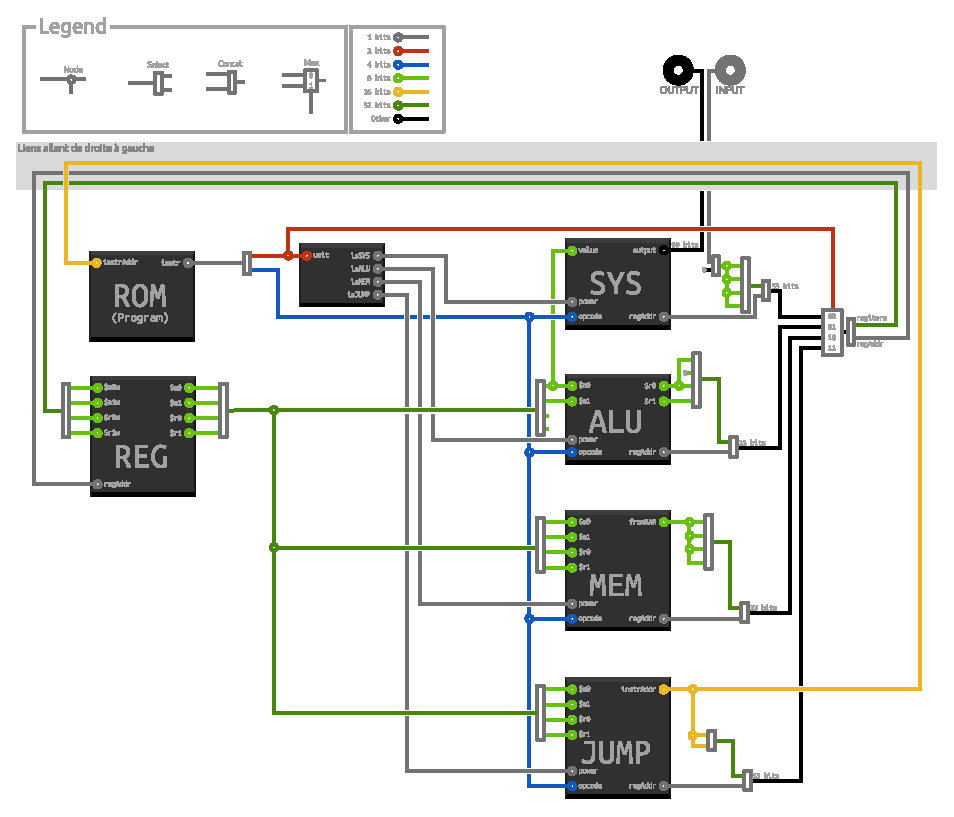
\includegraphics{archi.eps}
\caption{\label{archi} Architecture microprocesseur}
\end{figure}
\paragraph{}La figure \ref{archi} présente l'architecture microprocesseur et l'interaction
entre les différentes unités.


\subsubsection{GPU}
Derrière le module SYS se cache en fait un cinquième module : le GPU (\emph{Graphical Processing Unit}, je précise par principe bien que je me doute que vous en connaissiez le sens). Le GPU représente en nombre de portes la moitié de notre processeur et a pour rôle de convertir les entiers codés en binaire en une série de codages 7 segments. Le poids important de cette partie du circuit vient du fait qu'il doit gérer simultanément les 7 entiers affichés.

\paragraph{}Les deux actions les plus effectuées par le GPU sont les divisions euclidiennes par 10 et les conversions 4 bits binaires vers 7 segments (le comportement en cas de valeur supérieure à 9 n'étant pas spécifié). Nous avons tenté d'optimiser les divisions par 10, le diviseur étant connu statiquement, mais il s'est avéré que le nombre de portes n'était pas diminué. Il se peut que cette absence de différence entre la division générale et la division par une constante connue d'avance disparaisse lors de la phase d'optimisation du simulateur, mais nos tests datent d'avant l'existence de cette phase.

\paragraph{}La séparation CPU/GPU est un point très intéressant du circuit : il est central puisque le GPU représente la moitié du circuit, mais les liens entre les deux sont d'une part peu nombreux et d'autre part à sens unique. Cela nous a permis de couper la simulation en deux afin d'optimiser l'utilisation de processeurs multi-cœurs en lançant simplement deux occurences du simulateur.


\subsection{Ajout récent}
\label{micro_update}
Cette partie du microprocesseur n'était pas présente dans l'ancienne version rendue le 7 janvier mais s'est avéré être indispensable pour limiter le taille du programme.

\paragraph{}On a déjà remarqué que les premières adresses mémoire (de 0 à 7) sont relativement simple d'accès (un \emph{load immediat} suffit) alors que les adresses suivantes sont presque impossible à atteindre sans effacer presque tous les registres en pratique et donc inutilisables. L'idée que l'on a eu pour y remédier est d'ajouter un pseudo-registre, noté \$c, qui serait un curseur vers une adresse donnée de la RAM à partir duquel tous les accès mémoire se feraient. Un accès à l'adresse $x$ se fait ainsi en réalité à l'adresse \$c + $x$.

\paragraph{}Les opérations possibles sur ce pointeur \$c sont “ajouter 8” (INCR) et “retirer 8” (DECR), la valeur 8 correspondant au nombre d'adresses faciles d'accès. On enregistre en réalité $\frac{\$c}8$ étant donné que les 3 derniers bits sont toujours à 0. Cette méthode permet de limiter le nombre d'instructions à ajouter.

\paragraph{}Il devient ainsi très simple d'accéder aux adresses au-delà de 8, bien que le temps d'accès ne soit plus constant. On a également pu augmenter la taille de la RAM. Bien que ce système permette de gérer une RAM de taille quelconque, nous nous sommes contenté de $2^16 = 65536$ adresses. Notre programme n'utilise en réalité que 8 chunks (24 adresses) mais par soucis de généralité nous avons voulu montré qu'il était possible de gérer une grande quantité de RAM et donc d'envisager de compiler n'importe quelle programme vers notre assembleur, ce que 256 adresses ne permet pas vraiment.

\paragraph{}Notons que nous aurions pu choisir, au vu du son poids important, de gérer la logique du GPU directement dans l'afficheur. Mais nous tenions à jouer le jeu de la simulation jusqu'au bout et imaginer la sortie du simulateur directement branchée fil par fil aux 98 segments de l'afficheur.

\begin{figure}[h]
\centering
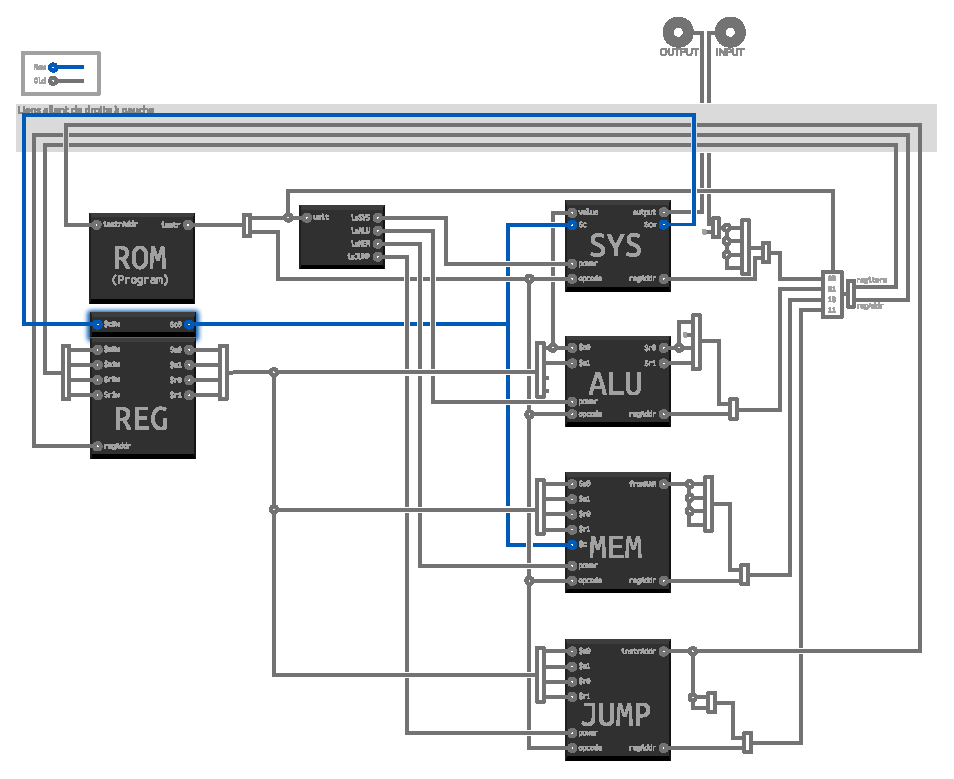
\includegraphics{archi_update.eps}
\caption{\label{archi_update} Architecture microprocesseur mise à jour}
\end{figure}
\paragraph{}La figure \ref{archi_update} met en évidence la modification approtée sur le schéma du microprocesseur. On peut noter que nous avons dû faire une entorse à notre partitions en différentes unités : le curseur \$c, bien que relatif aux accès mémoire, est géré par le module système. C'était le seul endroit où il subsistait des adresses d'instruction libres.


\subsection{Jeu d'instruction détaillé}

\begin{savenotes}
\begin{longtable}{|c|l|l|}
  
  \hline
  Code & Nom & Description \\
  \endfirsthead
  \hline
  Code & Nom & Description \\
  \hline\hline
  \endhead

  \hline\hline
  00 ** ** & \multicolumn{2}{|l|}{SYS} \\
  \hline
  00 00 10 & INCR    & Incrémente le curseur de bloc. \\
  00 00 11 & DECR    & Décrémente le curseur de bloc. \\
  \hline\hline
  00 01 00 & INPUT    & \'Ecrit l'input dans un registre donné. \\
  00 1* ** & OUTPUT x & \'Ecrit la valeur de \$a0 dans la mémoire graphique x, avec 0 $\leq$ x $\leq$ 7 \\
  00 11 11 & FLIP     & Actualise l'affichage du timer avec ce qu'il y a dans sa mémoire. \\
  
  \hline\hline
  01 ** ** & \multicolumn{2}{|l|}{ALU} \\
  \hline
  00 00 ** & \multicolumn{2}{|l|}{Arithmétique} \\
  \hline
  01 00 00 & ADD   & Ajoute \$a0 et \$a1. Le résultat est dans \$r0, la retenue dans \$r1. \\
  01 00 01 & SUB   & Soustrait \$a1 à \$a0. Le résultat est dans \$r0\footnote{$\$r0=\$a0-\$a1$ est certifié uniquement si $\$a0>\$a1$}, la retenue dans \$r1. \\
  01 00 10 & MULT  & Multiplie \$a0 et \$a1. Le résultat est dans la concaténation de \$r0 et \$r1.\\
  01 00 11 & DIV   & Divise \$a0 par \$a1. Le quotient est dans \$r0, et le reste dans \$r1. \\
  \hline
  00 01 ** & \multicolumn{2}{|l|}{Logique} \\
  \hline
  01 01 00 & AND   & Calcule le AND bit-à-bit de \$a0 et \$a1 dans \$r0. \\
  01 01 01 & OR    & Calcule le OR bit-à-bit de \$a0 et \$a1 dans \$r0. \\
  01 01 10 & NOT   & Calcule le NOT bit-à-bit de \$a0 dans \$r0, et de \$a1 dans \$r1. \\
  01 01 11 & SHIFT & SHIFT \$a0 de min(\$a1,n) vers les poids forts. Le résultat est dans la concaténation de \$r0 et \$r1.\\
  \hline
  01 1* ** & LI x  & Charge une constante x à trois bits\footnote{Le reste est rempli de 0} dans \$a0. \\
  
  \hline\hline
  10 ** ** & \multicolumn{2}{|l|}{MEM} \\
  \hline
  10 0* ** & \multicolumn{2}{|l|}{entre registres} \\
  \hline
  10 00 ij & MOVE 0ij & Déplace un \$a[i] vers un \$r[j]. \\
  10 01 ij & MOVE 1ij & Déplace un \$r[i] vers un \$a[j]. \\
  \hline
  10 1* ** & \multicolumn{2}{|l|}{avec la RAM} \\
  \hline
  10 10 ij & LOAD ij  & Charge la valeur en RAM(\$r[i]) dans \$a[j]. \\
  10 11 ij & SAVE ij  & Enregistre dans RAM(\$r[i]) la valeur \$a[j]. \\

  \hline\hline
  11 ** ** & \multicolumn{2}{|l|}{JUMP} \\
  \hline
  11 00 ij & JFRA ij & Ajoute \$[i][j] à l'adresse de lecture (saut en avant relatif). \\
  11 01 ij & JBRA ij & Retranche \$[i][j] à l'adresse de lecture (saut en arrière relatif). \\
  11 10 ij & IIO  ij & Saute une instruction si le registre donné est non nul. \\
  11 11 0i & JAA  i  & Saut à une adresse absolue donnée par \$[i]0.\$[i]1\\
  11 11 10 & WCA     & \'Ecrit l'adresse courante dans \$a0.\$a1. \\
  11 11 11 & END      & Termine le programme. \\
  \hline

\caption{Instructions microprocesseur}
\end{longtable}
\end{savenotes}

On peut constater qu'il manque 2 instructions dans ce tableau, les 2 premières.
La toute première, l'instruction 00 00 00, a volontairement été laissée inactive
car c'est la valeur que prennent toutes les cases de la ROM par défaut. Il était
important pour aider au déboguage qu'elle ne fasse rien et peut s'avérer utile
si on fait des sauts de taille approximative et que l'on a donc besoin d'ajuster,
ce qui peut être le cas lorsque l'on cherche à optimiser le code en profitant du
fait qu'une certaine valeur soit déjà chargée dans un registre.

\paragraph{}Pour l'instruction restante, elle ne fait rien non plus mais uniquement car
on ne lui a pas trouvé de rôle. Elle fait partie de l'unitée système et est trop
peu nombreuse pour ajouter par exemple une fonction de lecture des registres graphiques.
On ne pouvait lui donner de rôle sans aboutir à un jeu d'instruction complètement incohérent.


\subsection{Outils de développement}

\paragraph{}Le microprocesseur doit être décrit sous forme de netlist. On se rend cependant très vite compte en faisant quelques essais que rédiger directement en netlist est extrêmement fastidieux (et de fait, on manipulera par moment des netlist de près de 30 000 lignes). De nombreuses portions du code se répètent, certaines sont paramétriques et si on décide de changer la taille des mots machine par exemple on est bien embêté.

\paragraph{}C'est pourquoi il est impératif d'utiliser une description plus haut niveau. Il y a pour cela deux possibilités :
\begin{itemize}
	\item utiliser un programme générant directement la netlist pour le micro
	\item compiler en netlist depuis un langage de description de circuits plus haut niveau.
\end{itemize}

\paragraph{}Un compilateur minijazz étant fourni, nous avons choisi la seconde option. Ce choix a cependant posé plusieurs problèmes.

Premièrement, minijazz étant un langage très simple, il ne gère pas l'import de fichiers les uns dans les autres. Cette fonctionnalité nous semblait pourtant essentielle, d'une part pour pouvoir utiliser une même portion de circuit dans plusieurs tests distincts (par exemple le gpu et l'alu) et d'autre part pour pouvoir travailler sans se gêner sur le circuit (git gère bien mieux des fichiers séparés).

Deuxièmement, les messages d'erreur de mjc étaient assez obscures, que ce soit les « The following constraint is not satisfied: ((8 = 0) ? 1 : (8 = (((0 <= (8 - 1)) ? (((8 - 1) - 0) + 1) : 0) + ((0 <= (8 - 8)) ? (((8 - 8) - 0) + 1) : 0)))) » ou les erreurs localisées « Quelque part entre la première et la dernière ligne du fichier ». Le debogage consistait donc en une longue dichotomie sur tout le code du microprocesseur.





\section{Programme}

\section{Oscillateur}

\section{Afficheurs}






\end{document}
